\documentclass[11pt, a4paper]{article} %tamaño mínimo de letra 11pto.
%Packages en la plantilla:
\usepackage[english]{babel} %Español 
\usepackage[utf8]{inputenc} %Para poder poner tildes
\usepackage{vmargin} %Para modificar los márgenes
\setmargins{2.5cm}{1.5cm}{16.5cm}{23.42cm}{10pt}{1cm}{0pt}{2cm}
%margen izquierdo, superior, anchura del texto, altura del texto, altura de los encabezados, espacio entre el texto y los encabezados, altura del pie de página, espacio entre el texto y el pie de página
%Packages extra, a excepción de graphicx
\usepackage{physics}
%\bra{a'}\ket{b'}
%\bra*{a'}\ket*{b'} fixed size of bras and kets
%\bracket{a}{b} scalar product, also use \ip{}
%\bracket{a} a scalar a
%\ketbra{a}{b} outer product, also use \op{}
%\expval{A}{\Psi} expectation value, also use \ev
%\matrixel{n}{A}{m} or \mel for matrix element
\usepackage{amsmath, amssymb, bm}
\usepackage{caption}
\usepackage{graphicx}
\usepackage{fancyhdr}
\usepackage{kantlipsum}
\usepackage{appendix}
%for tables
\usepackage{multirow}
\usepackage{adjustbox}
\usepackage[table,xcdraw]{xcolor}
\usepackage{longtable}
\usepackage{colortbl}
\usepackage{rotating}
\usepackage{booktabs}
\usepackage{float}
\usepackage{wrapfig}
\usepackage{subcaption}
\usepackage{tcolorbox}
\usepackage[hidelinks]{hyperref}
\usepackage[backend=biber,sorting=none]{biblatex}
\usepackage{csquotes}

\usepackage{tcolorbox}

\addbibresource{repbib.bib}
%Bibliografia

%Introducir las imágenes en la carpeta images
\graphicspath{{images/}}
%\decimalpoint

\begin{document}
%%%%%%Portada%%%%%%%
\begin{titlepage}
\centering
{ \bfseries \Large UNIVERSIDAD COMPLUTENSE DE MADRID}
\vspace{0.5cm}

{\bfseries  \Large FACULTAD DE CIENCIAS FÍSICAS} 
\vspace{1cm}

{\large DEPARTAMENTO DE FÍSICA TEÓRICA}
\vspace{0.8cm}

%%%%Logo Complutense%%%%%
{
\includegraphics[width=0.35\textwidth]{logo_ucm}} %Para ajustar la portada a una sola página se puede reducir el tamaño del logo
\vspace{0.8cm}

{\bfseries \Large TRABAJO DE FIN DE GRADO}
\vspace{2cm}

{\Large Código de TFG:  FT-38 } \vspace{5mm}

{\Large Resonancias con varios quarks pesados}\vspace{5mm}

{\Large Resonances with several heavy quarks}\vspace{5mm}

{\Large Supervisor/es: Felipe J. Llanes Estrada}\vspace{20mm} 

{\bfseries \LARGE Mario Camilo Pardo Rodríguez}\vspace{5mm} 

{\large Grado en Física}\vspace{5mm} 

{\large Curso acad\'emico 2023-2024)}\vspace{5mm} 

{\large Convocatoria XXXX}\vspace{5mm} 

\end{titlepage}
\newpage

{\bfseries \large [Título extendido del TFG (si procede)] }\vspace{10mm} 

{\bfseries \large Resumen:} \vspace{5mm}

Esto es una prueba para probar el formato del Resumen. Esto es una prueba para probar el formato del ResumenEsto es una prueba para probar el formato del ResumenEsto es una prueba para probar el formato del ResumenEsto es una prueba para probar el formato del ResumenEsto es una prueba para probar el formato del ResumenEsto es una prueba para probar el formato del ResumenEsto es una prueba para probar el formato del ResumenEsto es una prueba para probar el formato del ResumenEsto es una prueba para probar el formato del ResumenEsto es una prueba para probar el formato del ResumenEsto es una prueba para probar el formato del ResumenEsto es una prueba para probar el formato del ResumenEsto es una prueba para probar el formato del ResumenEsto es una prueba para probar el formato del Resumen.
\vspace{1cm}

{\bfseries \large Abstract: }\vspace{5mm} 

This is a test to prove the abstract's layout.This is a test to prove the abstract's layout.This is a test to prove the abstract's layout.This is a test to prove the abstract's layout.This is a test to prove the abstract's layout.This is a test to prove the abstract's layout.This is a test to prove the abstract's layout.This is a test to prove the abstract's layout.This is a test to prove the abstract's layout.This is a test to prove the abstract's layout.This is a test to prove the abstract's layout.This is a test to prove the abstract's layout.This is a test to prove the abstract's layout.This is a test to prove the abstract's layout.This is a test to prove the abstract's layout.This is a test to prove the abstract's layout.This is a test to prove the abstract's layout.This is a test to prove the abstract's layout.This is a test to prove the abstract's layout.
\vspace{1cm}

%%Comentar estas notas para que no salgan en la memoria
{\Large\textbf{Nota: el título extendido (si procede), el resumen y el abstract deben estar en una misma página y su extensión no debe superar una página. Tamaño mínimo 11pto.}}
\vspace{1cm}

{\Large\textbf{Extensión máxima 20 páginas sin contar portada ni resumen (sí se incluye índice, introducción, conclusiones y bibliografía}}
\newpage
\tableofcontents
\newpage
%Beginning
%%Hartree_Fock:
\section{Hartree - Fock method}
When dealing with a stationary Schrödinger equation, an analytical solution can only be found for simplified, specific problems such as the hydrogen atom. For more complex problems, the idea of an exact solution is discarded and approximate methods are adopted. One of main importance is the variational method. In it, a set of solutions restricted to a subspace of the Hilbert space is proposed, and then a solution which minimises the energy functional (\ref{eq:energy_functional}) is found within the subspace.
\begin{equation}
    E\left[\psi\right] = \frac{\ev{H}{\psi}}{\ip{\psi}}
    \label{eq:energy_functional}
\end{equation}
Thus, under the Rayleigh-Ritz variational principle, the Hamiltonian expectation value from any ansatz wavefunction is an upper bound to the exact ground state energy \cite{griffiths,szabo}.\\\\
In the spirit of the variational method, the Hartree-Fock method is the approach to the many-body problem presented in this work. The aim of this procedure is to find the solution wave functions in the form of an anti-symmetrised product of one-electron wave functions.

\subsection{Preliminaries}\label{preliminaries}
\paragraph{Born - Oppenheimer approximation in atomic/molecular physics:}
When dealing with a system consisting of many electrons and nuclei, the starting Hamiltonian involves too many coupled degrees of freedom. In the first place, by knowing that the nuclei are much heavier than the electrons, one can assume that the former move more slowly than the latter. Thus, it is reasonable to assume a Hamiltonian for N electrons in the field generated by a static configuration of K nuclei (\ref{eq:BO_hamiltonian}), and therefore to consider the nuclear-nuclear repulsion to be constant for a given electronic configuration. This is the widely known Born-Oppenheimer approximation \cite{sutcliffe}. %TODO Check: Moreover, the kinetic energy of the nuclei can be neglected, such that the total energy of the system is given by the sum of the energy of the electrons and the electrostatic energy of the nuclei \cite{computationalphysics}.
With the Hartree-Fock procedure the electronic energy will be minimised. To find the ground state of the whole system and obtaining an \emph{adiabatic} potential for the electrons, the procedure must be repeated changing the positions of the nuclei.%TODO Check this last phrase
\begin{equation}
    H_{BO} =\sum_{i=1}^N\frac{p_i^2}{2}+
    \frac{1}{2} \sum_{i,j=1;i\neq j}^N \frac{1}{\left|\mathbf{r}_i -\mathbf{r}_j\right|} - 
    \sum_{n=1}^K\sum_{i=1}^N \frac{Z_n}{\left|\mathbf{r}_i -\mathbf{R}_n\right|}
    \label{eq:BO_hamiltonian}
\end{equation}
where atomic units have been used \cite{szabo}. It should be noted that the Born-Oppenheimer Hamiltonian omits some interactions such as spin-orbit and that it neglects quantum fluctuations.
\paragraph{Independent particle method:}
The interelectronic repulsion terms in (\ref{eq:BO_hamiltonian}) make impossible to find an eigenfunction of the Hamiltonian, since it is not separable. The main idea for solving this problem is by decoupling its terms with the independent particle method. This is, by considering that the interaction between an electron and the remaining ones can be incorporated in the Hamiltonian as if the remaining ones created an averaged electrostatic field on the electron. In this way, an uncoupled, effective Hamiltonian is obtained for each electron:
\begin{equation}
    H_{IP}=\sum_{i=1}^N\left[\frac{p_i^2}{2}+V(\mathbf{r_i})\right]=\sum_{i=1}^N h(i)
    \label{eq:IP_hamiltonian}
\end{equation}
where $V(\mathbf{r_i})$ is a potential dependent on the chosen configuration of the nuclei, usually a non-local operator. This independent particle Hamiltonian will be further discussed later on.\\\\
The fact that $H_{IP}$ is a sum of one-electron Hamiltonians makes it possible to find an eigenfunction as a product of spin orbital wave functions:
\begin{equation}
	\Psi (q_1,...,q_N) = \psi_1(q_1)... \psi_N(q_N)
	\label{eq:prod_spinorbitals}
\end{equation}
where $q = (\mathbf{r},s)$ contains the spatial and spin coordinates of one electron. This solution wave function may also be referred as a \emph{Hartree product}. The corresponding eigenvalue $E$ is then a sum of the spin orbital energies corresponding to each $\psi_k$: $E = \sum_{k=1}^N\epsilon_k$. 

It should be noted that a solution wave function of this form has an uncorrelated probability distribution, since the probability density of finding each particle $i$ in the volume element $d\mathbf{x}_i$, centred at $\mathbf{x}_i$, can be written as a product of the one-particle probability densities:
\begin{equation}
	\rho (q_1,...,q_N) = \left|\psi_1(q_1)\right|^2... \left|\psi_N(q_N)\right|^2
	\label{eq:prob_density}
\end{equation}
Therefore, a solution of this form distinguishes particles by the spin orbital they occupy. Nevertheless, for satisfying the antisymmetry principle, indistinguishability of electrons must be taken into account with an antisymmetric wave function. Hartree-Fock theory will fix this deficit.

\paragraph{Self-consistent-field (SCF)} Lets now search for an approximate independent particle Hamiltonian for the case of K nuclei and N electrons within the Born-Oppenheimer aproximation. For this introduction the antisymmetry requirement will not be taken into account, as the solution wave function will be chosen to have the form of a Hartree product.\\\\
In first place, the spin-independent Hamiltonian acting on the solution wave function reads:%TODO Jupyter_Levine citation? Hartree scf is not  directly used on spin-orbitals :(
\begin{equation}
    \left[-\sum_{i=1}^N\frac{1}{2}\nabla_i^2+
    \sum_{i,j=1;i\neq j}^N \frac{1}{\left|\mathbf{r}_i -\mathbf{r}_j\right|} - 
    \sum_{n=1}^K\sum_{i=1}^N \frac{Z_n}{\left|\mathbf{r}_i -\mathbf{R}_n\right|}\right]\Psi (q_1,...,q_N) = E \Psi (q_1,...,q_N)
    \label{eq:hart1}
\end{equation}
For separating this equation, such that an independent particle equation is obtained for each spin-orbital $\psi_k$, both sides of (\ref{eq:hart1}) can be multiplied from the left by $N-1$ spin orbitals\footnote{This is, multiplying by $\prod_{m\neq k}^N\psi_m^* (q_m)$.} $\psi_m^* (q_m)$ and integrated over every $q_m$, therefore arriving to%TODO Check N-1 or N
\begin{equation}
    \left[-\frac{1}{2}\nabla^2 - 
    \sum_{n=1}^K \frac{Z_n}{\left|\mathbf{r} -\mathbf{R}_n\right|} + 
    \sum_{l=1}^N \int{dq'\left|\psi_l(q')\right|^2\frac{1}{\left|\mathbf{r} -\mathbf{r'}\right|}}\right]\psi_k (q) = E' \psi_k (q)
    \label{eq:hart2}
\end{equation}
where normalisation of the spin orbitals is assumed and several constants have been absorbed into the new variable $E'$. The third term on the left hand side will be referenced later on as the Hartree potential, which represents the Coulomb energy of the $k$-th electron in the average field generated by the charge distribution caused by all the N electrons\footnote{A usual nuisance is the self-coupling of the $k$-th electron. Hartree-Fock theory will solve this problem by taking into account the antisymmetry requirement of the wave function.}.

One can see that the Hamiltonian acting on $\psi_k$ in this equation has the form of an effective one-electron Hamiltonian $h(i)$. In this way, an independent particle equation (\ref{eq:IP_hamiltonian}) has been obtained. %In addition, $V(\mathbf{x})$ can be identified as a non-local operator, since it depends on the unknown solution wave function.\\\\%It is worth noting that this could be done because the wave function is a product of spin orbitals.
%TODO Thanks to prod of spin-orb
%TODO Non-local operator?
For finding the spin-orbitals the \textbf{Hartree self-consistent-field method} shall be used \cite{Blinder}. For doing so, a trial ground state solution $\psi^{(0)}$ is proposed for constructing the potential. Then, solving the spin orbital equations (\ref{eq:hart2}) yields an improved ground state $\psi^{(1)}$, which is then used to build a new potential. This procedure is repeated until convergence is met\footnote{Different criteria may be used for checking convergence. For example, the ground state not deviating appreciably between iterations. This will be further discussed when the Hartree-Fock computer program is presented.}.

\paragraph{Antisymmetry and correlation} %For finding a solution wave function that can satisfy the antisymmetry principle it is fundamental to remember that electrons are identical particles. This means that the Hamiltonian commutes with the particle-exchange operator

Any valid wave function must be antisymmetric with respect to particle exchange. To extend the Hartree product of equation (\ref{eq:prod_spinorbitals}) to satisfy the antisymmetry principle, an antisymmetric linear combination of the spin orbitals can be used. A usual such ansatz is the Slater determinant
\begin{equation}
	\Psi (q_1,...,q_N)= \frac{1}{\sqrt{N!}}
	\begin{vmatrix}
  \psi_1 (q_1) & \psi_2 (q_1) & \cdots & \psi_N (q_1)\\
  \psi_1 (q_2) & \psi_2 (q_2) & \cdots & \psi_N (q_2)\\
  \vdots & \vdots & \ddots & \vdots \\
  \psi_1 (q_N) & \psi_2 (q_N) & \cdots & \psi_N (q_N)
\end{vmatrix}
\end{equation}
From now on, a more convenient, simplified notation for a normalized Slater determinant will be used \cite{szabo}:
\begin{equation}
		\Psi (q_1,...,q_N) \equiv \ket{\psi_1(q_1)... \psi_N(q_N)}\equiv\ket{\psi_1... \psi_N}
\end{equation}
It should be noted that antisymmetrisation introduces correlation effects, which can be seen by considering the probability density of finding two electrons with coordinates $q_1$ and $q_2$:
\begin{equation}
	\rho(q_1, q_2) = \frac{1}{N(N-1)}	\sum_{k,l}\left[\left|\psi_k(q_1)\right|^2\left|	\psi_l(q_2)\right|^2-\psi_k^*(q_1) 	\psi_k(q_2) \psi_l(q_1) \psi_l^*(q_2)\right]
	\label{eq:correlated_prob}
\end{equation}
%Lets consider spin orbitals that can be written as a product of a spatial orbital and a one-particle spin wave function, i.e. $\psi_k(\mathbf{x}_k) = \chi_k(\mathbf{r}_k)\alpha(\omega_k)$. 
From this it can be deduced that correlation exchange is only present for equal spin orbitals, whereas opposite spin orbitals remain uncorrelated (as they do in equation (\ref{eq:prob_density})). Moreover, if electrons have parallel spin and $\mathbf{r}_1= \mathbf{r}_2$, then $\rho(q_1, q_1)=0$, thus satisfying Pauli's exclusion principle. %TODO ref.
For this it is said that the electrons are surrounded by an \emph{exchange} or \emph{Fermi hole}, in which other electrons with the same spin are hardly found \cite{szabo,computationalphysics,slater1}.
%TODO Want to justify it or just reference computational? If just reference, then do the same when explaining non-correlation. Review scf. If only the citation, explain qualitatively (szabo)
%%%%%%%%%%%%%%%%%%%%%%%%%%%%%%%%%%%%%%%%%%%%%%%%%%%%%%%%%%%%%%%
\subsection{Hartree-Fock theory}
%La herramienta principal que se emplea para resolver el problema de varios cuerpos es el método de Hartree - Fock, fundamental en el estudio de átomos polielectrónicos y moléculas.\\\\
%Se considera en primer lugar el hamiltoniano de un sistema de $N$ electrones y $K$ núcleos \cite{computationalphysics}.]

%SEE modern-quantum-chemistry 2.2
%The Hartree-Fock approximation is proposed for dealing with the many-body problem, and consists on reducing it to several single-body problems, in which the interelectronic repulsion is incorporated in an average way. As it's been presented, Hartree did this for the Coulomb repulsion. For taking antisymmetry into account, 
V.A. Fock extended the Hartree equation by including a nonlocal term, the exchange contribution. The Hartree - Fock equations read \cite{szabo,mcweeny}: 
\begin{equation}
	\mathcal{F}\psi_k = \varepsilon_k \psi_k,
	\mathrm{where}
	\label{eq:short_HF}
\end{equation}
\begin{multline}
	\mathcal{F}\psi_k = \left[-\frac{1}{2}\nabla^2 - \sum_n\frac{Z_n}{\left|\mathbf{r}-\mathbf{R}_n\right|}\right]\psi_k(q) + \sum_{l=1}^N\int{dq'\left|\psi_l(q')\right|^2\frac{1}{\left|\mathbf{r}-\mathbf{r'}\right|}\psi_k(q)} -\\ -\sum_{l =1}^N\int{dx'\psi_l^*(q')\frac{1}{\left|\mathbf{r}-\mathbf{r'}\right|}\psi_k(q')\psi_l(q)}
	\label{eq:Hartree_Fock}
\end{multline}

$\mathcal{F}$ is called the Fock operator. The terms within brackets build up the uncoupled one-electron Hamiltonian $h$. The third (Coulomb) and fourth (exchange) terms compose the Hartree-Fock potential, and respond to the interelectronic interaction. This potential depends on the Fock operator's eigenfunctions $\psi_k$. Therefore, the problem is non-linear and must be solved with the self-consistency-field method introduced in subsection \ref{preliminaries}. %A few comments seem necessary. 

It should be noted that the eigenvalues $\varepsilon_k$ %are Lagrange multipliers and
do not represent the energies of single electron orbitals. However, they provide the total energy
\begin{equation}
    E = \sum_{k=1}^N\left[\ev{\psi_k \left| h\right| \psi_k}+\ev{\psi_k \left|\frac{1}{2}(\tilde{J}-\tilde{K}) \right| \psi_k}\right]=\nonumber\frac{1}{2}\sum_{k=1}^{N}\left(\varepsilon_k+\mel{\psi_k}{h}{\psi_k}\right)
    \label{eq:energies_heps}
\end{equation}
where $\tilde{J}$ and $\tilde{K}$ represent the Coulomb and exchange operators respectively. This expression can be easily deduced by comparing the expected value of the Born-Oppenheimer Hamiltonian (\ref{eq:BO_hamiltonian}) with the Hartree-Fock equation (\ref{eq:Hartree_Fock}).\\\\
%TODO
%For readability purposes, a more thorough explanation on (\ref{eq:energies_heps}) and the upcoming energy expressions is presented in the appendix \ref{appendix:energies}.

%It must be noted as well that the auto-coupling problem presented in the Hartree equation (\ref{eq:hart2}) is solved by including the exchange operator, since the Hartree-Fock potential vanishes for $k=l$.

%Finally, in the derivation of (\ref{eq:short_HF}) it is assumed that the solution wave function is restricted to the space of single Slater determinants, i.e. when dealing with a closed-subshell system or a system with one electron outside the closed subshells. If this is not the case, the Hartree-Fock equations happen to be more complicated \cite{computationalphysics, jupyter_levine}.\\\\
%TODO Koopman's theorem
For the purpose of this work only closed-shell systems will be studied, which means that all occupied levels are completely filled by two electrons with opposite spin. In this way, all spin orbitals can be grouped by pairs with common orbital dependence and opposite spin \cite{computationalphysics}. Calculations within this constrain are called \emph{restricted Hartree-Fock} (RHF).

This is specially useful for the Hartree-Fock equation (\ref{eq:Hartree_Fock}), since the Fock operator does not depend \textbf{explicitly} on the spin. Then, an operator which only depends on spatial orbitals can be found. By summing over the spin degrees of freedom an equivalent Hartree-Fock equation is derived
\begin{equation}
	F(\mathbf{r})\phi(\mathbf{r}) = \left(h(\mathbf{r})+2J (\mathbf{r})-K (\mathbf{r})\right)\phi (\mathbf{r})=\varepsilon\phi (\mathbf{r})
	\label{eq:new_HF}
\end{equation}
with $J (\mathbf{r}) $ and $K (\mathbf{r}) $ representing the (redefined) Coulomb and exchange operators respectively
\begin{align}
	J (\mathbf{r})\phi (\mathbf{r}) &= 2 \sum_{l=1}^{N/2}\int{d^3r'\left|\phi_l(\mathbf{r'})\right|^2\frac{1}{\left|\mathbf{r}-\mathbf{r'}\right|}\phi(\mathbf{r})}\\
	K (\mathbf{r})\phi (\mathbf{r}) &= \sum_{l =1}^{N/2}\int{d^3r'\phi_l^*(\mathbf{r'})\phi (\mathbf{r'})\frac{1}{\left|\mathbf{r}-\mathbf{r'}\right|}\phi_l (\mathbf{r})}
	\label{eq:coulomb_exchange}
\end{align}
where $\phi_l$ represent the spatial part of the ansatz wave functions.
Note that the sums run only to $N/2$ because of the previous sum over the spin degrees of freedom. From now on, sums over $k$ will be considered to extend to all different spatial orbitals (this is, half of the total number of orbitals). Thus, the ground state energy is given by
%\begin{equation}
%    E = 2\sum_k\mel{\phi_k}{h}{\phi_k}+\sum_k\left(2\mel{\phi_k}{J}{\phi_k}-\mel{\phi_k}{K}{\phi_k}\right)= \sum_k \left[\varepsilon_k + \mel{\phi_k}{h}{\phi_k}\right],
%\end{equation}
an analog expression to (\ref{eq:energies_heps}) except for a factor $2$.%where $\varepsilon_k$ are the eigenvalues of the redefined Fock operator $F$.  



\subsection{Hartree-Fock computer program}
In this section the general structure of a Hartree-Fock computer program will be presented. Its flow chart can be found in figure \ref{fig:flowchart}, whereas in Appendix \ref{appendix:code} the \emph{Fortran} implementation is given. To check its validity, the ground state energy yielded for the helium atom and the hydrogen molecule will be compared with the bibliography at the end of the section.
\begin{enumerate}
    \item \textbf{Input data:} The first step in every Hartree-Fock program should be to present the problem to be solved. For this, the number of electrons $N$, the atomic numbers $Z_n$ and nuclei positions $\mathbf{R}_n$ must be introduced. If various nuclei are present in the problem, calculating the bond lengths or angles could be desired. If so, the following steps must be repeated for every nuclear configuration.
    %Nosense to include next paragraph if Roothaan is not used
    %Moreover, a certain basis set must be chosen for the specific problem. Most common basis sets are Slater type orbitals (STO), Gaussian type orbitals (GTO) and linear combinations of them. Several basis sets can be found at \cite{basissetexchange}.

    \item \textbf{Calculate matrices:} All matrices which do not depend on the density matrix can be determined before entering the SCF loop. These are the overlap matrix $S_{pq}$, the uncoupled one-electron hamiltonian $h_{pq}$ and the two-electron integrals $\mel{pr}{g}{qs}$. For efficiency purposes, it should be taken into account that $S_{pq}$ and $h_{pq}$ are symmetric matrices, so that only $N(N+1)/2$ elements should be calculated. More importantly, the two-electron integrals respond to several symmetries: $p\longleftrightarrow q\;; \; \; r\longleftrightarrow s\;; \; \; p,q\longleftrightarrow r,s$. This way, roughly $N^4/8$ elements should be calculated \cite{computationalphysics}.

    In this step internuclear repulsion shall as well be calculated.

    \item \textbf{Bring overlap matrix to unit form:} For transforming the Roothaan equation to a standard eigenvalue equation, it is relevant to bring the overlap matrix to unit form. Also, this way one assures that the eigenvectors yielded by the equation are normalised via the overlap matrix. For bringing the overlap matrix to unit form, a transform matrix \textbf{X} is defined such that $\mathbf{X}^\dagger \mathbf{S}\mathbf{X} = \mathbf{I}$. 
    
    \begin{tcolorbox}[colback=blue!5!white,colframe=blue!1!white]
        In this work the method of symmetric orthogonalisation will be considered, where $\mathbf{X}=\mathbf{S}^{-1/2}$. For finding the desired transformation matrix, the overlap matrix must be diagonalised first. This is, finding a unitary matrix $\mathbf{U}$ which satisfies $\mathbf{U}^\dagger\mathbf{S}\mathbf{U} = \mathbf{s}$, where $\mathbf{s}$ is the diagonalised overlap matrix. Since the overlap matrix's eigenvalues are always positive \cite{computationalphysics}, one can define its \emph{inverse square root} as a matrix with the inverse square root of the eigenvalues on the diagonal. From this follows transforming back the transformation matrix:
        \begin{equation}
            \mathbf{X} = \mathbf{S}^{-1/2} = \mathbf{U} \mathbf{s}^{-1/2} \mathbf{U}^\dagger
        \end{equation}
        and the transformation matrix $\mathbf{X}$ can then be easily obtained by diagonalising $\mathbf{S}$.
    \end{tcolorbox}
    \item \textbf{First guess for the density matrix:} For building the Fock matrix, a first guess for the density matrix must be done. It happens to be a reasonably good choice for most cases to neglect interelectronic interaction in the first iteration, such that the Fock matrix is identical to the uncoupled one-electron Hamiltonian $h$. By looking back at (\ref{eq:fock_matrix}) one can see that this is equivalent to considering all elements $P_{rs}=0$.
    \item \textbf{SCF loop:} Once the relevant matrices are built, the self consistent field method is applied by finding new density matrices until convergence is met.
    \begin{enumerate}
        \item \textbf{Calculate the electron-electron repulsion matrix:} The Coulomb and exchange contribution to the Fock matrix can be stored, altogether with the density matrix, in an \emph{electron-electron repulsion matrix} $\mathbf{G}$, such that $F_{pq}=h_{pq}+G_{pq}$:
    \begin{equation}
        G_{pq} = \sum_{r,s}P_{rs}\left[\mel{pr}{g}{qs}-\frac{1}{2}\mel{pr}{g}{sq}\right]
        \label{eq:two_electron_matrix}
    \end{equation}
    This way, the Fock matrix can be easily calculated. It should be noted that accessing the two-electron integrals can be a very time-consuming process for the computer. To improve this one can introduce a Yoshimine sort algorithm \cite{yoshimine}.%, or by simply storing the matrix elements with their corresponding indices.
    \item \textbf{Solve the Roothaan equation:} The transformation matrix which brings $\mathbf{S}$ to unit form is useful for transforming the Roothaan equation $\mathbf{F C}=\varepsilon\mathbf{S C}$ to an ordinary eigenvalue equation. Then, the resulting eigenvectors can be transformed back and used for building the new density matrix. The structure is as follows:
        \begin{tcolorbox}[colback=orange!5!white,colframe=orange!1!white]%orange!135black
            Multiplying the Roothaan equation (\ref{eq:roothaan_equation}) with $\mathbf{X}^\dagger$ from the left and introducing the identity $\mathbf{X}\mathbf{X}^{-1}=\mathbf{I}$,
            \begin{equation}
                \mathbf{X}^\dagger\mathbf{F}\  \mathbf{X}\mathbf{X}^{-1} \mathbf{C} = \varepsilon \mathbf{X}^\dagger\mathbf{S}\  \mathbf{X}\mathbf{X}^{-1}\mathbf{C}
            \end{equation}
            which immediately delivers the desired ordinary eigenvalue equation:
            \begin{align}\label{eq:transformed_roothaan}
                \mathbf{F}'\mathbf{C}'&=\varepsilon\mathbf{C}',\mathrm{where}\\
                \mathbf{F}'&=\mathbf{X}^\dagger\mathbf{F}\mathbf{X}\ \mathrm{and}\nonumber\\
                \mathbf{C}'&=\mathbf{X}^{-1}\mathbf{C}\nonumber.
            \end{align}
            Now, transforming back the eigenvectors can be easily done, as $\mathbf{C} = \mathbf{X}\mathbf{C}'$.
        \end{tcolorbox}
    \item \textbf{Build a new density matrix:} The new density matrix can be calculated by its definition in (\ref{eq:density_matrix}), with the eigenvectors yielded by the Roothaan equation (\ref{eq:transformed_roothaan}).
    \item \textbf{Check for convergence:} For achieving convergence Fock levels must not deviate much from one iteration to another. If convergence is not met, the SCF loop is repeated, taking the new density matrix as input.\\\\Some systems may not satisfy this convergence criteria though. In this case, instead of using the calculated density matrix for the next iteration, a weighted average between iterations can be used \cite{computationalphysics}.
    \end{enumerate}
    \item \textbf{Calculate the ground state energy:} If convergence is met, the energy can be obtained as
    
    \begin{align}
	    	E &= \sum_{p,q}^MP_{pq} h_{pq} + \frac{1}{2}\sum_{p,q,r,s}^M P_{pq}P_{rs}\left[\mel{pr}{g}{qs}-\frac{1}{2}\mel{pr}{g}{sq}\right]+E_{nuc}\nonumber\\
    	&= \frac{1}{2}\sum_{p,q}^MP_{pq} h_{pq}+\sum_k \varepsilon_k + E_{nuc}
    		\label{eq:energy_computer}
    \end{align}
    where $P_{pq}$ are the elements of the new density matrix, $\varepsilon_k$ is the eigenvalue representing the k-th Fock level and $E_{nuc}$ is the repulsion energy between the nuclei for the given configuration.
\end{enumerate}
    






\newpage
\newpage
\appendix
\section*{Appendix}
\addcontentsline{toc}{section}{Appendix}
\renewcommand{\thesubsection}{\Roman{subsection}}
\subsection{Code}
\label{appendix:code}
\begin{figure}[H]
    \centering
    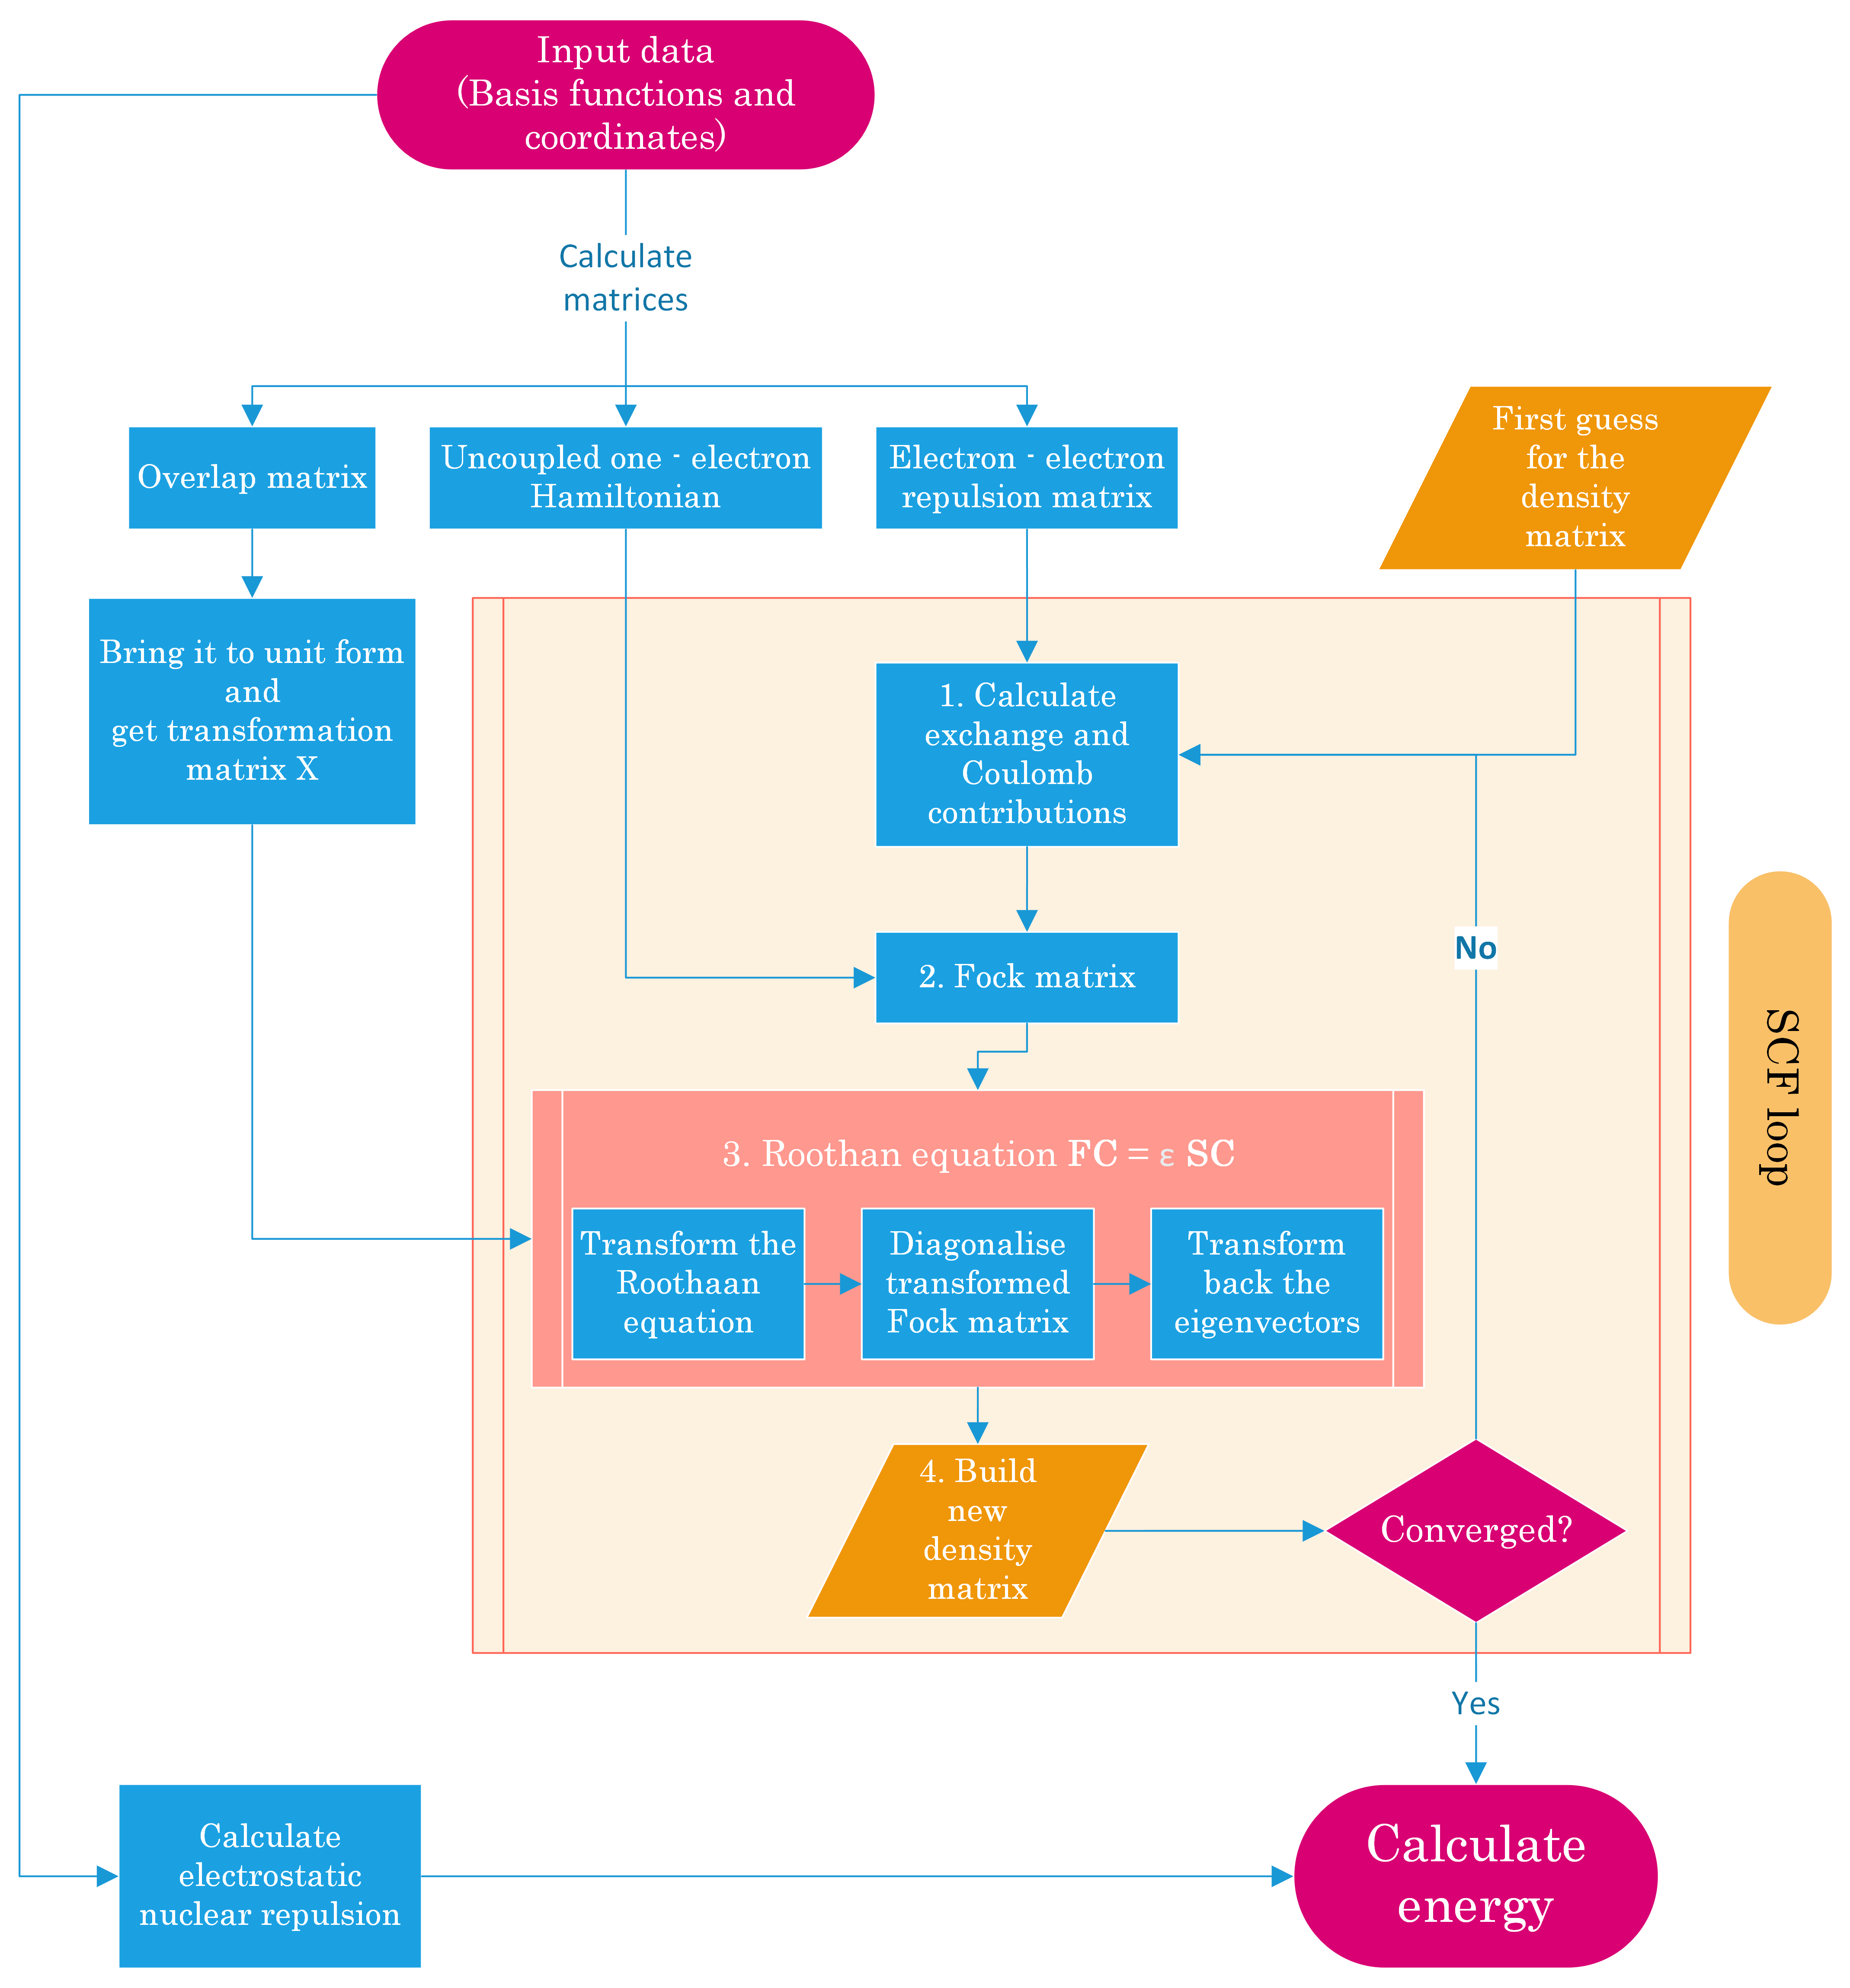
\includegraphics[width = \textwidth]{HF_flowchart}
    \caption{Flow chart of a Hartree-Fock program.}
    \label{fig:flowchart}
\end{figure}
\subsection{On the energy expression derivation}\label{appendix:energies}
The expression of the energy can be obtained, as usual, by calculating the expectation value of the Hamiltonian. Assuming the use of a single Slater determinant and within the frame of the Born-Oppenheimer approximation, the Hamiltonian (\ref{eq:hart1}) has the form
\begin{align}\label{eq:hamiltonian_derivation}
    &H=\sum_i^N h(i)+\frac{1}{2}\sum_{i,j;i\neq j}^Ng(i,j),\; \; \mathrm{where}\\
    &h(i)=-\frac{1}{2}\nabla_i^2-
\sum_{n=1}^K \frac{Z_n}{\left|\mathbf{r}_i -\mathbf{R}_n\right|}\; \; \mathrm{and}\nonumber\\
    &g(i,j) = \frac{1}{\left|\mathbf{r}_i -\mathbf{r}_j\right|}.\nonumber
\end{align}
By taking $\psi$ to be the Slater determinant of a Hartree product, and introducing the notation:
\begin{equation}
    \mel{\psi_k \psi_l}{g}{\psi_m\psi_n} = \int{d\mathbf{x_1}d\mathbf{x_2}\psi_k^*(\mathbf{x_1})\psi_l^*(\mathbf{x_2})\frac{1}{\left|\mathbf{r}_i -\mathbf{r}_j\right|}\psi_m(\mathbf{x_1})\psi_n(\mathbf{x_2})}
\end{equation}
one can get the expectation value of the energy as
\begin{equation}
    E = \sum_k^N\mel{\psi_k}{h}{\psi_k}+\frac{1}{2}\sum_{k,l}^N\left(\mel{\psi_k \psi_l}{g}{\psi_k\psi_l}-\mel{\psi_k \psi_l}{g}{\psi_l\psi_k}\right).
    \label{eq:unsimple_energy}
\end{equation}
Moreover, by defining the Coulomb and exchange operators respectively:
\begin{align}
    J=\sum_k^NJ_k& : J_k(\mathbf{x})\psi(\mathbf{x})=\int{d\mathbf{x}'\psi_k^*(\mathbf{x})' \frac{1}{\left|\mathbf{r}_i -\mathbf{r}_j\right|}\psi_k(\mathbf{x}')\psi(\mathbf{x})}\\
    K=\sum_k^NK_k& : K_k(\mathbf{x})\psi(\mathbf{x})=\int{d\mathbf{x}'\psi_k^*(\mathbf{x})'\frac{1}{\left|\mathbf{r}_i -\mathbf{r}_j\right|} \psi(\mathbf{x}')\psi_k(\mathbf{x})}
\end{align}
the energy functional has the simpler form
\begin{equation}
    E=\sum_k^N\ev{\psi_k \left| h + \frac{1}{2}(J-K) \right| \psi_k}
    \label{eq:energy_hJK}
\end{equation}
Now, by defining the Fock operator
\begin{equation}
    \mathcal{F}=h+J-K
\end{equation}
which satisfies the eigenvalue equation
\begin{equation}
    \mathcal{F}\psi_k   = \varepsilon_k\psi_k,
\end{equation}
the relationship between the eigenvalues $\varepsilon_k$ and the energy (\ref{eq:energy_hJK}) can be obtained as follows:
\begin{align}
    E &= \sum_k^N\left[\ev{\psi_k \left| h\right| \psi_k}+\ev{\psi_k \left|\frac{1}{2}(J-K) \right| \psi_k}\right]=\nonumber\\&=\sum_k^N\left[\varepsilon_k-\ev{\psi_k \left|\frac{1}{2}(J-K) \right| \psi_k} \right]=\sum_k^N\left[\varepsilon_k+\mel{\psi_k}{h}{\psi_k} \right]-E\Leftrightarrow\nonumber\\&\Leftrightarrow E=\frac{1}{2}\sum_k^N\left[\varepsilon_k+\mel{\psi_k}{h}{\psi_k} \right]
    \label{eq:energyobtained}
\end{align}
which can be identified as the expression presented in the work (\ref{eq:energies_heps}).\\\\
After redefining the Fock, Coulomb and exchange operators for the spatial orbitals such that the Fock equation reads $F = h+2J-K$  ---see equation (\ref{eq:new_HF})---, the energy is given by an analogous expression to (\ref{eq:energy_hJK}):
\begin{equation}
    E = 2\sum_k^{N/2}\mel{\phi_k}{h}{\phi_k}+\sum_k^{N/2}\left(2\mel{\phi_k}{J}{\phi_k}-\mel{\phi_k}{K}{\phi_k}\right)
\end{equation}
As it is presented in the work, from now on it will be assumed that sums over $k$ extend to all different spatial orbitals (this is, half of the total number of orbitals, $N/2$).

Now, by introducing the parametrisation 
\begin{equation}
    \phi_k=\sum_{q}^MC_{qk}\chi_q(\mathbf{r})
    \label{eq:parametrisation}
\end{equation}
the energy can be written as
\begin{equation}
    E = \sum_{p,q}^MP_{pq} h_{pq} + \frac{1}{2}\sum_{p,q,r,s}^M P_{pq}P_{rs}\left[\mel{pr}{g}{qs}-\frac{1}{2}\mel{pr}{g}{sq}\right]
\end{equation}
where $\mathbf{P}$ is the density matrix defined in (\ref{eq:density_matrix}) and $\mel{pr}{g}{qs}$ represent a two-electron integral using the notation presented in (\ref{eq:g_matrix}).

Moreover, an equivalent expression dependent on the Fock levels ---the eigenvalues $\varepsilon_k$ of the new Fock operator $F$--- can be found:
\begin{align}
    \sum_k \varepsilon_k &= \sum_k\left[\mel{\phi_k}{h}{\phi_k}+2\mel{\phi_k}{J}{\phi_k}-\mel{\phi_k}{K}{\phi_k}\right]\nonumber\\
    &=\sum_k\mel{\phi_k}{h}{\phi_k} + E - 2\sum_k\mel{\phi_k}{h}{\phi_k} = E - \sum_k\mel{\phi_k}{h}{\phi_k}\Leftrightarrow\nonumber\\
    &\Leftrightarrow E = \sum_k \left[\varepsilon_k + \mel{\phi_k}{h}{\phi_k}\right]
\end{align}
which, again, by introducing the parametrisation (\ref{eq:parametrisation}) and the density matrix,
\begin{equation}
    E = \frac{1}{2}\sum_{p,q}^MP_{pq} h_{pq}+\sum_k \varepsilon_k
\end{equation}
It should be remembered that the total energy of the system shall include as well the internuclear repulsion energy for the given configuration.
\newpage

\printbibliography[heading=bibintoc]
\end{document}

